\documentclass{article}
\usepackage[utf8]{inputenc}

\title{BDSA - Assignment0 Description}
\author{Jacob Møller Jensen}
\date{September 2021}

\usepackage{natbib}
\usepackage{graphicx}
\usepackage[colorlinks = true,
            linkcolor = blue,
            urlcolor  = blue,
            citecolor = black,
            anchorcolor = blue]{hyperref}
\usepackage[margin=1in]{geometry}

\begin{document}

\maketitle

\section*{IsLeapYear Diagram}

\begin{figure}[h!]
\centering
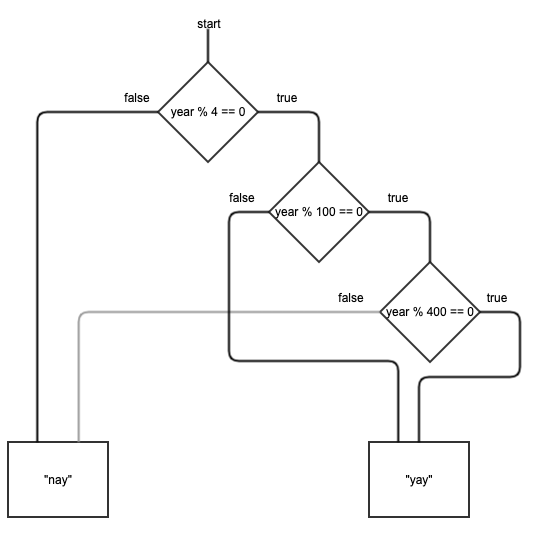
\includegraphics[scale=0.5]{media/Assignment0diagram2}
\caption{Diagram visualising the algorithm used in the IsLeapYear function.}
\label{fig:media/Assignment0diagram2}
\end{figure}
\section*{IsLeapYear Description}
This algorithm uses 3 checks to see whether the user-entered year is a leap year. For it to be a leap year it must be exactly dividable by 4, except for years that are devidable by 100. Only if they are both devidable by 100 and 400, they will be a leap year wich is the centurial leap years. 
\\\\
The algorithm checks these conditions in the order they were mentioned above in three if-statements. If they at any given time fails to match this pattern the code will return \textit{false}, meaning that it is not a leap year and the Console outputs \textit{"nay"}. Otherwise the code will contrariwise return \textit{true} and output \textit{"yay"}. The diagram shows the options at any state under which the year is checked with the modulo operator to see if a division returns zero as a remainder.

\end{document}
